\section{Deployment}

The deployment pipeline of the recommendation system involves setting up the Triton Ensemble and the external components of the system as shown in Figure \ref{fig:DeploymentDiagram}.
To use a Triton inference server, a Triton Ensemble has to be compiled with the necessary models, workflows, and configurations.

\subsection{Feast Materialization}

In order to use Feast as the feature store, the user and item features have to be materialized, 
meaning that they have to be moved from Feast's offline store, which in this case is a Parquet file, to its online store, which is a Redis database.

\subsection{Compiling Ensemble}

After the user and item features are materialized, the Triton Ensemble is compiled with all the models, workflows, and configurations.
Once compiled with all the components shown in Figure \ref{fig:DeploymentDiagram}, it outputs a directory tree similar to the one shown in Figure \ref{fig: EnsembleDirectoryTree}.

\begin{figure}[H]
    \centering
    \begin{subfigure}{.31\textwidth}
        \centering
        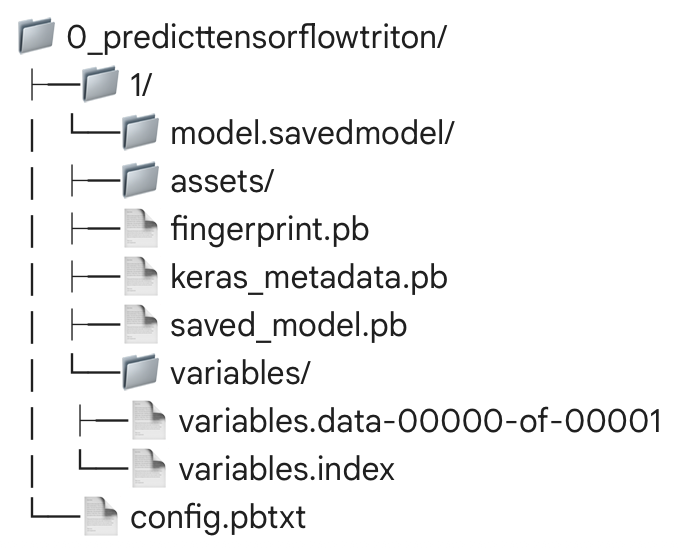
\includegraphics[width=\textwidth]{assets/ensemble_0.png}
        \label{fig:Ensemble0}
    \end{subfigure}
    \begin{subfigure}{.25\textwidth}
        \centering
        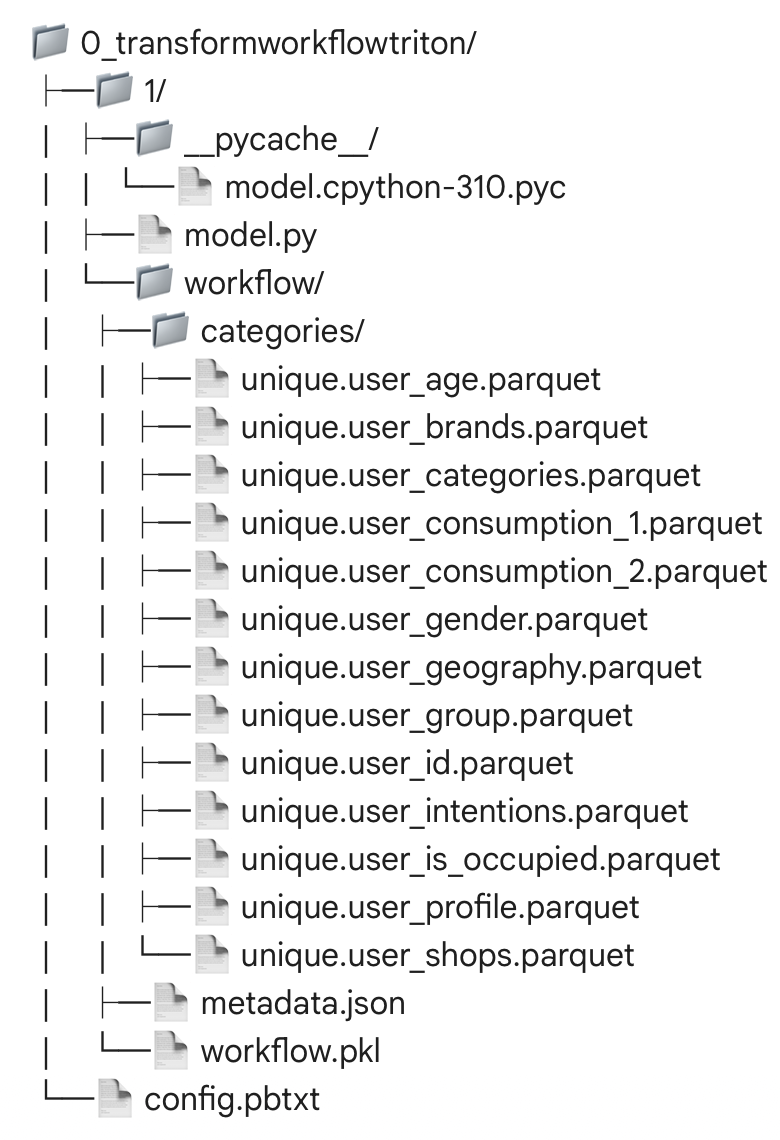
\includegraphics[width=\textwidth]{assets/ensemble_1.png}
        \label{fig:Ensemble1}
    \end{subfigure}
    \begin{subfigure}{.3\textwidth}
        \centering
        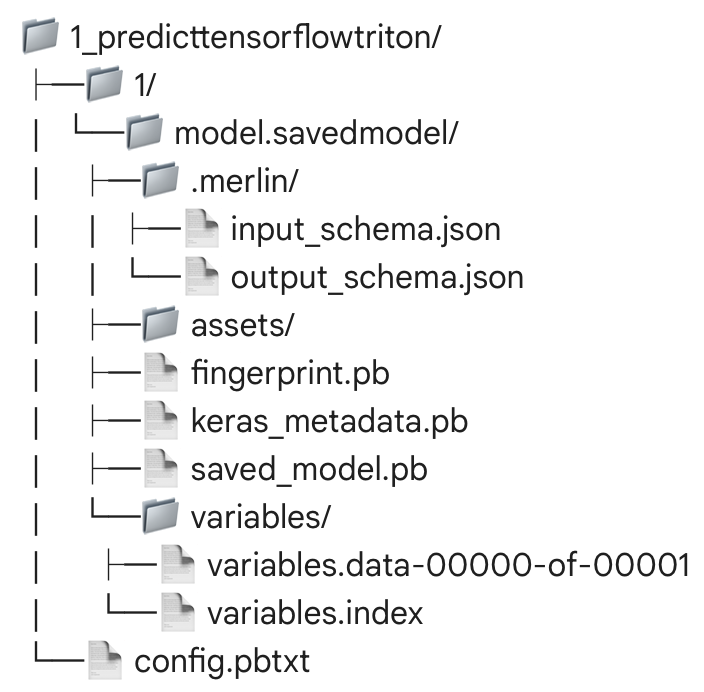
\includegraphics[width=\textwidth]{assets/ensemble_2.png}
        \label{fig:Ensemble2}
    \end{subfigure}
    \bigskip
    \begin{subfigure}{.3\textwidth}
        \centering
        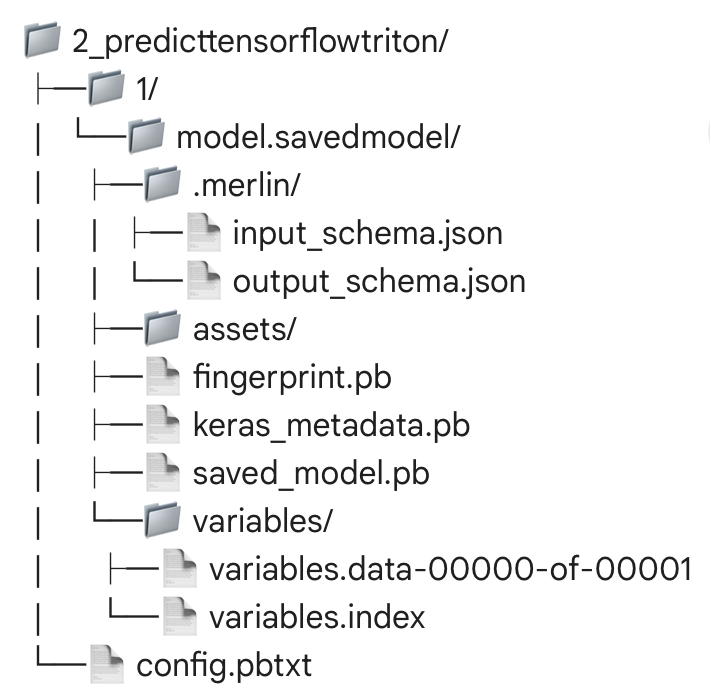
\includegraphics[width=\textwidth]{assets/ensemble_3.png}
        \label{fig:Ensemble3}
    \end{subfigure}
    \begin{subfigure}{.3\textwidth}
        \centering
        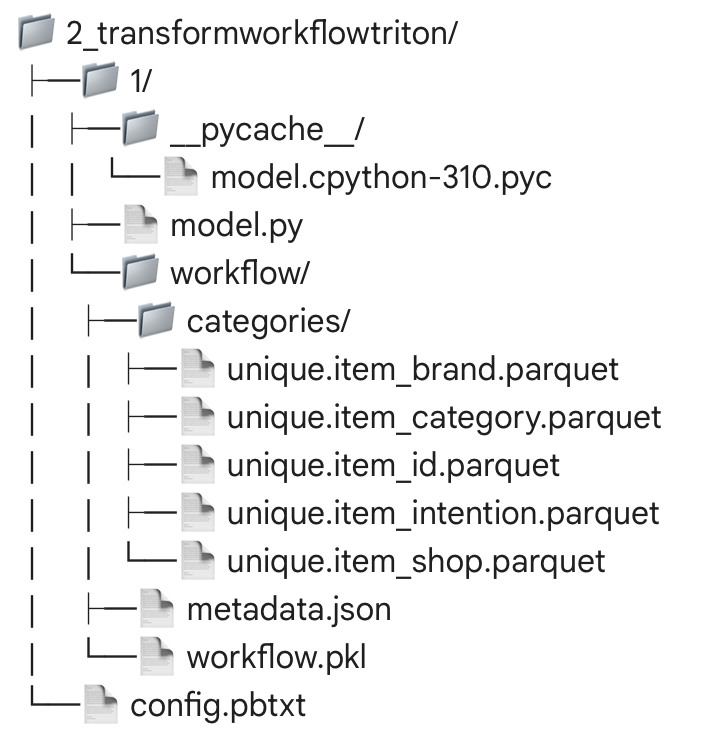
\includegraphics[width=\textwidth]{assets/ensemble_4.png}
        \label{fig:Ensemble4}
    \end{subfigure}
    \begin{subfigure}{.3\textwidth}
        \centering
        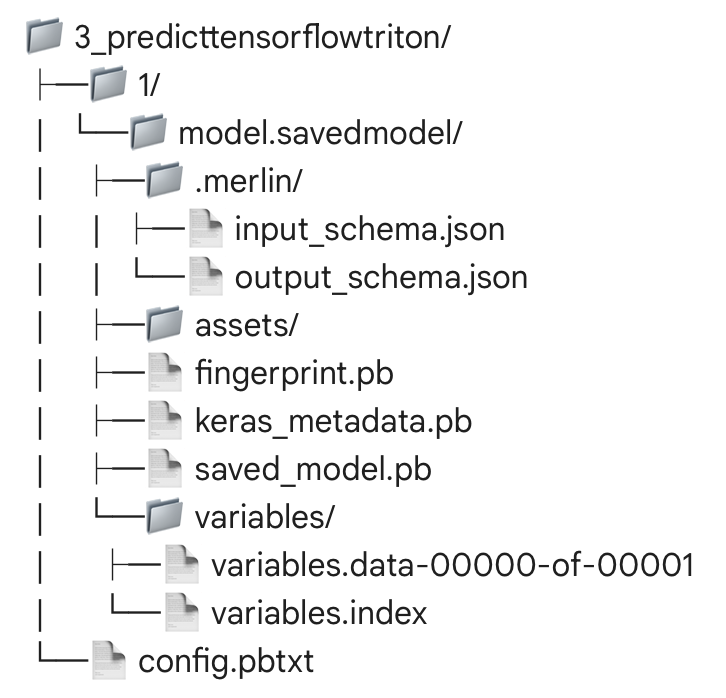
\includegraphics[width=\textwidth]{assets/ensemble_5.png}
        \label{fig:Ensemble5}
    \end{subfigure}
    \caption{Ensemble Directory Tree}
    \label{fig: EnsembleDirectoryTree}
\end{figure}


As shown in Figure \ref{fig: EnsembleDirectoryTree}, the Triton Ensemble directory tree contains model configurations, model weights, embeddings categories, and other necessary files.
Those files are saved to the model repository.

\section{API (TO REVISIT)}

TODO add api specification, performance benchmarks, and a better response list

\begin{figure}[H]
    \centering
    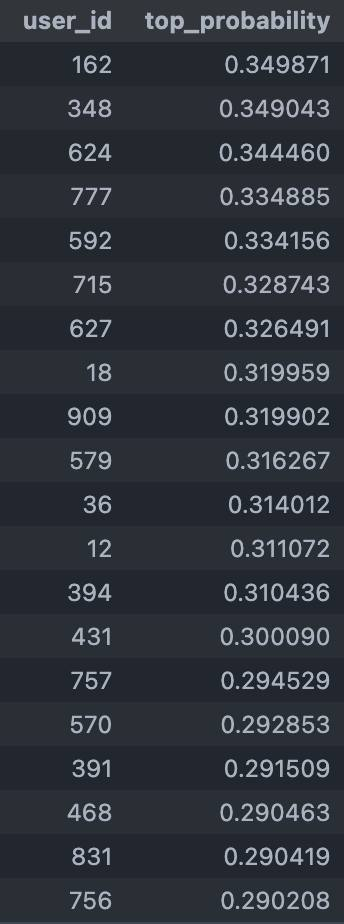
\includegraphics[width=0.4\textwidth]{assets/response_list.jpg}
    \caption{Response List TODO}
    \label{fig:ResponseList}
\end{figure}


\section{Performance Benchmarks TODO }
